
\documentclass{beamer}
\usepackage{graphicx}
\usepackage{float}
\usepackage{hyperref}
\usepackage{ulem}

\hypersetup{
colorlinks=true,
linkcolor=blue,
filecolor=magenta,
urlcolor=cyan,
}

\urlstyle{same}

\title{Presentation}
\date{\today}
\author{Your Name Here}
\begin{document}
\frame{\titlepage}

\begin{frame}
    \frametitle{Title of slide 1}

You can put regular text paragraphs here. Moreover, you can \textbf{bold your text} or \emph{italicize it} very
easily. Alternatively, you can use bullet points:


\begin{itemize}
\item Item 1
\item Item 2

\begin{itemize}
\item Item 2.2

\begin{itemize}
\item Item 2.2.1

\end{itemize}
\item Item 2.3

\end{itemize}

\end{itemize}


You can also write equations as you would in latex

$$
e^{i \pi} - 1 = 0
$$


\end{frame}


\begin{frame}
    \frametitle{Title Slide 2}


    \begin{figure}
        \centering
        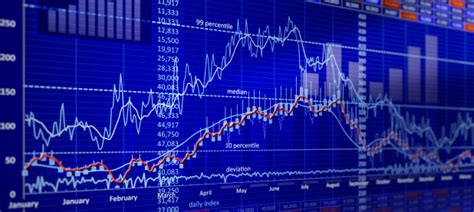
\includegraphics[width=0.9\paperwidth,height=0.7\paperheight,keepaspectratio]{./figs/stock_image.jpg}
        \caption{You can fullscreen pictures with captions!}
    \end{figure}
\end{frame}


\begin{frame}
    \frametitle{Pictures with text are automatically vertically split}

	\begin{minipage}{0.4\textwidth}
When you have a picture with text on the same slide, the area is automatically split.
\begin{itemize}
\item Margins can easily be adjusted in .tex file

\end{itemize}

	\end{minipage}%
	\hfill
	\begin{minipage}{0.55\textwidth}

    \begin{figure}
        \centering
        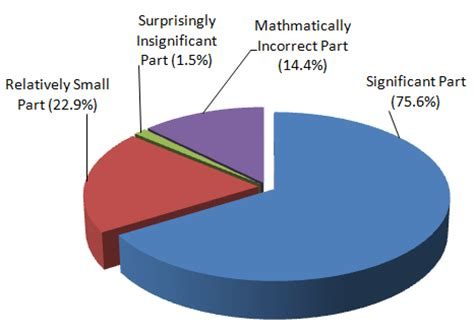
\includegraphics[width=\textwidth]{./figs/pie_chart.jpg}
        \caption{Anoter figure caption here!}
    \end{figure}	\end{minipage}

\end{frame}



\end{document}